%%%%%%%%%%%%%%%%%%%%%%%%%%%%%%%%%%%%%%%%%
% University Assignment Title Page 
% LaTeX Template
% Version 1.0 (27/12/12)
%
% This template has been downloaded from:
% http://www.LaTeXTemplates.com
%
% Original author:
% WikiBooks (http://en.wikibooks.org/wiki/LaTeX/Title_Creation)
%
% License:
% CC BY-NC-SA 3.0 (http://creativecommons.org/licenses/by-nc-sa/3.0/)
%
%%%%%%%%%%%%%%%%%%%%%%%%%%%%%%%%%%%%%%%%%
%\title{Title page with logo}
%----------------------------------------------------------------------------------------
%	PACKAGES AND OTHER DOCUMENT CONFIGURATIONS
%----------------------------------------------------------------------------------------

\documentclass[12pt]{article}
\usepackage[english]{babel}
\usepackage[utf8]{inputenc}
\usepackage{natbib}
\usepackage{amsmath}
\usepackage{color}
\usepackage[explicit]{titlesec}
\usepackage[hyphens,spaces,obeyspaces]{url}
\usepackage{graphicx}
\usepackage{caption}
\usepackage{subcaption}
\usepackage{grffile}
\usepackage{listings}
\usepackage{placeins}

\usepackage{booktabs}
\usepackage{tabularx}

\begin{document}

\begin{titlepage}

\newcommand{\HRule}{\rule{\linewidth}{0.5mm}} % Defines a new command for the horizontal lines, change thickness here

\center % Center everything on the page
 
%----------------------------------------------------------------------------------------
%	HEADING SECTIONS
%----------------------------------------------------------------------------------------

\textsc{\LARGE University of St Andrews}\\[1.5cm] % Name of your university/college
\textsc{\Large Distributed Systems}\\[0.5cm] % Major heading such as course name
\textsc{\large CS4103}\\[0.5cm] % Minor heading such as course title

%----------------------------------------------------------------------------------------
%	TITLE SECTION
%----------------------------------------------------------------------------------------

\HRule \\[0.4cm]
{ \huge \bfseries Ring-Based Distributed System}\\[0.4cm] % Title of your document
\HRule \\[1.5cm]
 
%----------------------------------------------------------------------------------------
%	AUTHOR SECTION
%----------------------------------------------------------------------------------------


\Large \emph{Author:}\\
 \textsc{150008022}\\[1cm] % Your name
 
%----------------------------------------------------------------------------------------
%	DATE SECTION
%----------------------------------------------------------------------------------------

{\large \today}\\[2cm] % Date, change the \today to a set date if you want to be precise

%----------------------------------------------------------------------------------------
%	LOGO SECTION
%---------------------------------------------------------------------------------------


\includegraphics[width = 4cm]{images/standrewslogo.png}
 
%----------------------------------------------------------------------------------------

\vfill % Fill the rest of the page with whitespace

\end{titlepage}

\section*{Goal}

To demonstrate an understanding of leader election and mutual exclusion in distributed systems by developing a ring-based distributed social media application.

\tableofcontents
\newpage

\pagenumbering{arabic}
\setcounter{page}{1} 

\section{Initial Set-up}

Java 8 was chosen for this project due to it's friendly socket API, and Maven \cite{maven} was used as the build tool. 

Since each node would be running on an isolated machine, the planned testing environment would involve using \emph{ssh} to start the nodes remotely. Providing the configuration as command line arguments was considered simpler than other methods, and was implemented using the Apache Commons CLI library \cite{apachecli}. 


In order to run the program, the arguments shown in table \ref{tbl:arguments} had to be specified. The purpose of each argument is explained later.

\renewcommand{\arraystretch}{1.5}
\begin{table}[!ht]
\centering
\begin{tabular}{ll}
\multicolumn{2}{l}{usage: java -jar $\langle$program$\rangle$.jar}
\\ 

 -d,--drop           &  Include if this node should trigger a database refresh. \\
 -e,--election $\langle$arg$\rangle$ &  Election method to use. \\
 -f,--list $\langle$arg$\rangle$     &  Path to file containing list of nodes (resource P). \\
 -i,--id $\langle$arg$\rangle$       &  ID of this node. 
\end{tabular}
\caption{Arguments for running application.}
\label{tbl:arguments}
\end{table}


\section{Ring Formation}

\subsection{Messages}

In order for nodes to understand and parse the messages that were sent between them, a message protocol was designed. Figure \ref{fig:mainmsg} shows the header that would be part of every message sent. The possible types of messages are summarised in table \ref{tbl:messagetypes}.

\begin{table}[!h]
\centering
\resizebox{\textwidth}{!}{%
\begin{tabular}{@{}lll@{}}
\toprule
Message Type                               & Usage                                                                                                                        & Payload                  \\ \midrule
\multicolumn{1}{l|}{JOIN}                  & \multicolumn{1}{l|}{Sent by new node to coordinator when wanting to join ring.}                                              & None                     \\
\multicolumn{1}{l|}{SUCCESSOR}             & \multicolumn{1}{l|}{Sent by coordinator to inform a node to connect to a new successor.}                                     & New Successor ID\\
\multicolumn{1}{l|}{SUCCESSOR\_REQUEST}    & \multicolumn{1}{l|}{Sent by a node to the coordinator after its successor has failed in order to be reassigned a successor.} & None                     \\
\multicolumn{1}{l|}{TOKEN}                 & \multicolumn{1}{l|}{Sent by a node to its successor.}                                                                        & None                     \\
\multicolumn{1}{l|}{TOKEN\_ACK}            & \multicolumn{1}{l|}{Sent by a node to its predecessor after receiving the token to confirm its reception.}                   & None                     \\
\multicolumn{1}{l|}{COORDINATOR\_ELECTION} & \multicolumn{1}{l|}{Message payload contains an election message.}                                                           & Election Message         \\ \bottomrule
\end{tabular}%
}
\caption{Possible values for the type field in the message header, with their usage and payload.}
\label{tbl:messagetypes}
\end{table}

The messages consist of serialized Java objects, which requires that they all implement the \emph{Serializable} interface. A more versatile format such as JSON would be preferred, but since all nodes would be using Java this method of serializing messages was kept. Figure \ref{fig:mainmsg} shows the header of every message, and figure \ref{fig:elecmsg} shows the header for an election message. 

\begin{figure}[!h]
\centering
\begin{minipage}{.5\textwidth}
  \centering
  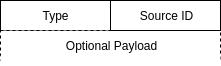
\includegraphics[width=.8\linewidth]{images/mainmsg}
  \captionof{figure}{Main message header.}
  \label{fig:mainmsg}
\end{minipage}%
\begin{minipage}{.5\textwidth}
  \centering
  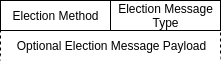
\includegraphics[width=.8\linewidth]{images/elecmsg}
  \captionof{figure}{Election message header.}
  \label{fig:elecmsg}
\end{minipage}
\end{figure}

The election message header would be in the payload of the main message. This allowed multiple election methods to be used and easy routing of election related messages to an election handler class.

\subsection{Communication}

Due to different patterns of communication during recovery and regular message passing phases both TCP and UDP were used for this project, as shown in Figure \ref{fig:pattern}.

\noindent TCP was used for communication \textbf{around} the ring:
\begin{enumerate}
    \item Reliable communication avoids token being lost.
    \item Connection is reused frequently between predecessors and successors, justifying handshake overhead.
\end{enumerate}

\noindent UDP was used for communication \textbf{across} the ring: 
\begin{enumerate}
    \item Low communication overhead allows for messages to be sent to multiple nodes quickly, improving recovery time from node failure.
    \item No session maintenance allows coordinator to handle more members in the ring.
    \item Multicast communication possible which would greatly simplify broadcasting.
\end{enumerate}

\subsection{Initialization}

On initialization, each node sends out join messages to the coordinator. The
joining protocol is similiar to that described in \cite{join}, and is shown in Figure \ref{fig:join}.
Figure \ref{fig:bigjoin} shows how the state of each connection changes over the course of
the joining procedure.

\begin{figure}[!ht]
\centering
  \centering
  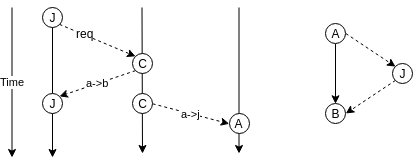
\includegraphics[width=.6\linewidth]{images/join}
  \caption{Joining protocol over time, with topology shown on right.}
\label{fig:join}
\end{figure}

\begin{figure}[!ht]
  \centering
  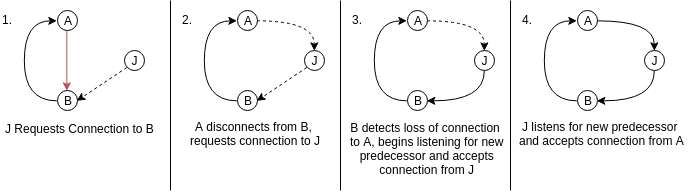
\includegraphics[width=\linewidth]{images/bigflow}
  \caption{State of each connection as a new node joins the ring. The red arrow
shows the edge that is replaced with the new node, and solid and dashed
arrows represent ongoing and pending connections respectively. Either A or
B can be the coordinator in this scenario.}
\label{fig:bigjoin}
\end{figure}
\FloatBarrier

\noindent When node J wants to join the ring:
\begin{enumerate}
    \item J sends join request to coordinator C.
    \item C sends successor to J, telling it to connect to B.
    \item C sends successor to A, telling it to connect to J. 
    \item A disconnects from B, B begins listening for new predecessor.
    \item J connects to B, A connects to J.
\end{enumerate}

In order for this process to work for a ring network with a single node,
it required another thread to wait on the connection, and the main thread
would then request the connection to itself. For two nodes and more the
joining node would be able to first connect to its new successor once its
predecessor had disconnected from its old successor as shown in figure \ref{fig:bigjoin}. 

\subsection{General Node Recovery}

When designing a distributed system, it should be assumed that failure will occur, and so as an extension this implementation included a mechanism for recovering from failure. Node failure is detected by either:
\begin{enumerate}
	\item a node attempting to read the socket connected to its predecessor.
	\item a node forwarding the token to its successor and not receiving an acknowledgement within a given timeframe.
\end{enumerate}

When a failure is detected by the successor of a failing node, it will simply begin listening for a new predecessor. Once the predecessor of the failing node detects the loss of connection, it will request a new successor from the coordinator node. The coordinator will then reply with the ID of the node after the failed node for the original predeccessor to connect to, at which point normal network behaviour can resume. Figure \ref{fig:failure} shows the topology change when a node fails.

\begin{figure}[!ht]
	\centering
	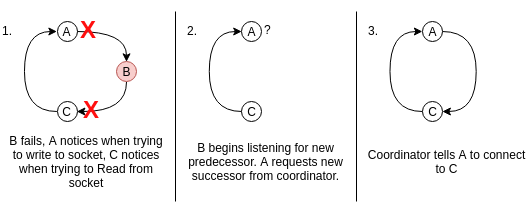
\includegraphics[width=\linewidth]{images/failure}
	\caption{Network topology during the recovery from node B failing. Either A or C are the coordinator in this scenario.}
	\label{fig:failure}
\end{figure}

The token acknowledgement message is the only occurence of communication in the reverse direction of the ring topology. The predecessor of the failing node will hold onto the token until it is assigned a new successor, and only releases the token once it has received the acknowlegement from it. This limits the number of situtations that can result in the loss of the token. If somehow the token is acknowledged but the acknowledgement message does not reach the predecessor in time, it could be possible for two tokens to then be in circulation. 

During testing, an edge case was realised with this recovery mechanism. If the disconnect is discovered when reading from the predecessor socket, there is a case where just waiting for a new predecessor does not work. Figure \ref{fig:hard} shows two scenarios where the disconnect is realised while reading from the predecessor socket. 

The scenario on the left would require A to first designate itself as its new successor before performing the self connection procedure described in the initialization protocol. This would only be necessary if the network consisted of two nodes, otherwise another node would eventually connect to A. The scenario on the right however is not one where an actual failure has occurred, and instead A is just changing its predecessor from itself to B. In order to check that the disconnect had occurred not because of failure, the token ring socket class (\emph{RingCommunicationHandler}) provided a boolean flag that would be true if the most recent disconnect had occurred while connected to itself. 

Knowing this meant that it could be assumed if there were only two nodes in the network that the other node has failed, and so a self connection would have to be performed as described in the previous section.

\begin{figure}[!ht]
	\centering
	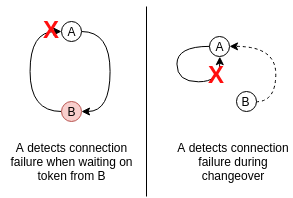
\includegraphics[width=0.6\linewidth]{images/hard}
	\caption{Two predecessor disconnect scenarios that are identical to the thread polling the predecessor socket.}
	\label{fig:hard}
\end{figure}

\subsection{Ring Topology Persistence}

Initially, the coordinator node was always the node with the ID 6. This node would maintain an in-memory virtual representation of the network topology using a cyclic linked list of node IDs. This obviously would be useless if the coordinator was to change, and so it was necessary to persist the network topology somehow. 

This was achieved by adding a database which would behave like resource P in the practical specification (the list of nodes). Only the coordinator would be able to write and update the database, and all other nodes would read from it. The database allowed operations to be carried out as transactions, meaning that node failure during an update could be rolled back. The database is initialized using a csv file containing the ID, address, and port of each node that \emph{may} join the network at some point. Figure \ref{fig:er} shows an ER diagram of the database schema. The successorId is nullable and refers to another row in the node table. If a value is present in that column then the node ID on that row would be assumed to be part of the ring.

\begin{figure}[!ht]
	\centering
	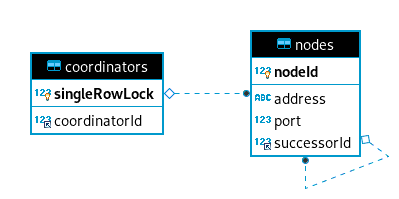
\includegraphics[width=0.6\linewidth]{images/er}
	\caption{ER diagram of the database schema for persisting the network topology.}
	\label{fig:er}
\end{figure}

When a new node wants to join the network, it first queries the database to learn who the current coordinator is. If no coordinator exists and no nodes have successors set, then this node will assume coordinator status. A limitation of this functionality is that if another node (B) queries for the current coordinator before the first node (A) has had the chance to update the database, then B could potentially also designate itself as coordinator. Since B would overwrite A as coordinator, later joining nodes would always make requests to B, and A would remain connected to itself.

The database was also essential for recovering the network topology quickly when a coordinator failed. If a node detected the failure of its successor and knew that its successor was currently the coordinator, it would temporarily act as a coordinator until a new one was elected. This would allow it to update the database and recover the ring topology by connecting to the successor of the failed coordinator. Immediately after recovering this connection, an election would be triggered by the acting coordinator in order to designate a permanent coordinator.

In order to ensure that only one coordinator existed at any time, the coordinators table included a boolean column \emph{singleRowLock} that would always be true. By setting this boolean column as the primary key, insert statements could then be constructed to either 
\begin{enumerate}
	\item Insert a new row if no coordinator exists with the value TRUE for \emph{singleRowLock}.
	\item Change the value of the coordinator ID if a row already exists by using the 'ON DUPLICATE KEY UPDATE' statement in the INSERT statement.
\end{enumerate}

Whilst another row could be added with the value FALSE for \emph{singleRowLock}, permissions would be configured such that only the hosts and a system administrator would be able to perform updates so it could be assumed that as long as the application code always used TRUE for inserts, only one row would ever exist. 


\section{Leader/Coordinator Election}

Firstly the ring-based election algorithm was implemented, as required for the basic specification. An interface was used for providing a generic 'election algorithm' API, allowing different algorithms to be switched out easily. Any messages that arrived from either the UDP socket or the ring sockets that were related 

\section{Receive/Send Posts}

\bibliographystyle{unsrt}
\bibliography{mybib}

\end{document}
